\chapter{Raw Evaluation Data}
\label{cha:rawdata}

\section{Additional Performance Benchmark Plots}
\label{cha:rawdata:performance}

	\autoref{img:rawdata:loss-vms-rails},
	\ref{img:rawdata:throughput-frameworks-mri22}, and
	\ref{img:rawdata:throughput-frameworks-jruby9} were kept out of
	\autoref{cha:evaluation:performance}, because they do not add significant
	information to the analysis. They are included in the appendix for the sake
	of completeness.

	\begin{figure}[H]
		\begin{center}
			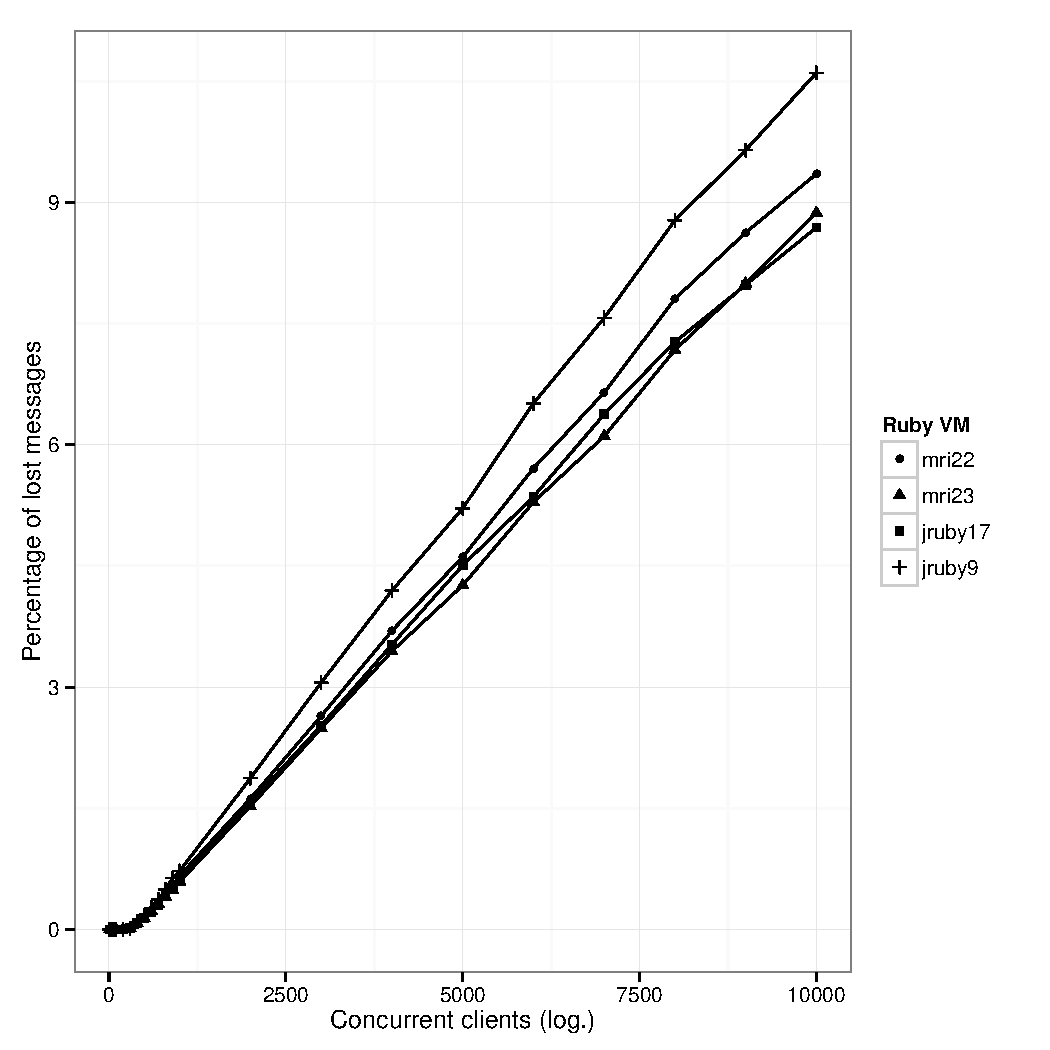
\includegraphics[width=\textwidth]{images/loss-vms-rails.pdf}
		\end{center}
		\caption{Message timeouts by Ruby \ac{VM} with \ac{Rails}}
		\label{img:rawdata:loss-vms-rails}
	\end{figure}

	\begin{figure}[H]
		\begin{center}
			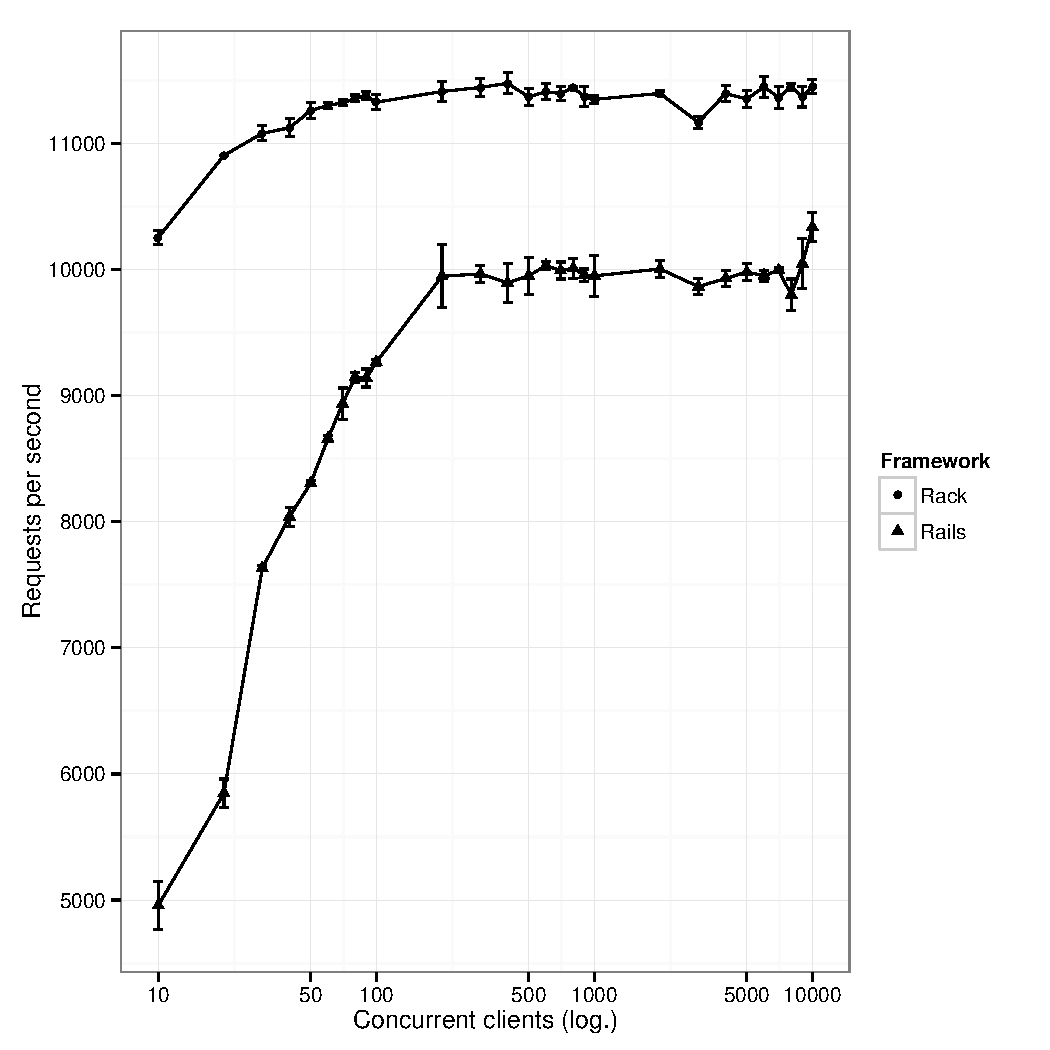
\includegraphics[width=\textwidth]{images/throughput-frameworks-mri22.pdf}
		\end{center}
		\caption{Throughput by Framework in \ac{MRI} 2.2.0p0}
		\label{img:rawdata:throughput-frameworks-mri22}
	\end{figure}

	\begin{figure}[H]
		\begin{center}
			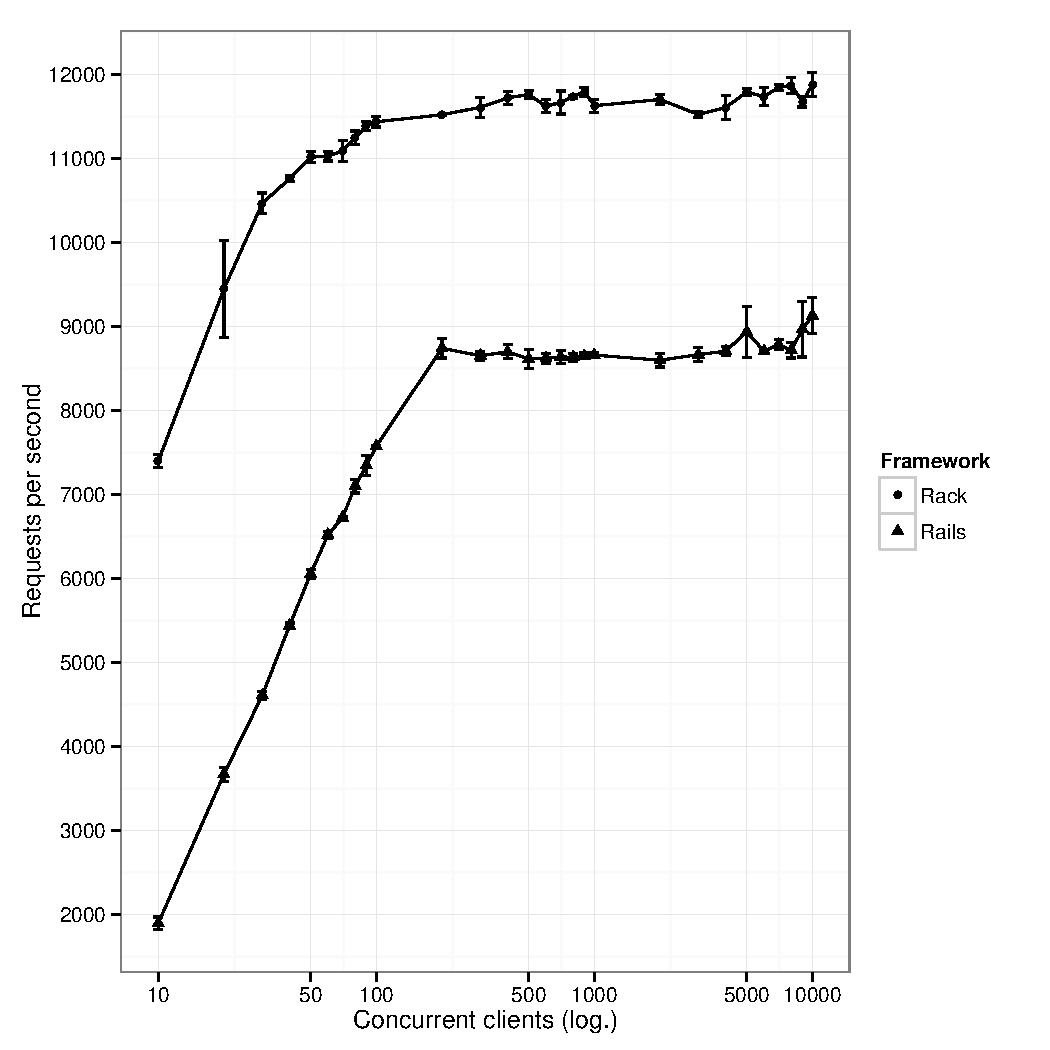
\includegraphics[width=\textwidth]{images/throughput-frameworks-jruby9.pdf}
		\end{center}
		\caption{Throughput by Framework in JRuby 9.0.0.0-pre1}
		\label{img:rawdata:throughput-frameworks-jruby9}
	\end{figure}

\section{Performance Benchmark on Ubiquiti EdgeMAX Lite}
\label{cha:rawdata:ubiquiti}

	\subsection{Router Preperations}

		\subsubsection{Firmware Update}

			\begin{itemize}
				\item Reset
				\item Firmware update to EdgeOS 1.6.0 (2014-11-05, Debian wheezy)
			\end{itemize}

		\subsubsection{Web Interface}

			After the reset the router has the IP address \texttt{192.168.1.1}
			on the first ethernet interface. Both login and password for the
			webinterface is \texttt{ubnt}. The performed configuration steps
			are:

			\begin{itemize}
				\item DHCP client on eth0 and eth2
				\item Deactivation of DHCP server and NAT
			\end{itemize}

	\subsection{Installing Ruby and git}

		\subsubsection{SSH and Root Shell}

			\begin{lstlisting}[gobble=8]
				ssh ubnt -l ubnt
				sudo -s
			\end{lstlisting}

		\subsubsection{Software Repositories}

			Both Debian stable and testing repository sources are needed.

			\begin{lstlisting}[gobble=8,caption={/etc/apt/sources.list.d/stable.list}]
				deb http://ftp.de.debian.org/debian/ stable main contrib non-free
				deb http://security.debian.org/ stable/updates main contrib non-free
			\end{lstlisting}

			\begin{lstlisting}[gobble=8,caption={/etc/apt/sources.list.d/testing.list}]
				deb http://ftp.de.debian.org/debian/ testing main contrib non-free
				deb http://security.debian.org/ testing/updates main contrib non-free
			\end{lstlisting}

			After configuring the package sources, \texttt{apt-get update} has
			to be executed.

		\subsubsection{Install Packages}

			The installation of git and essential tools to compile gems written
			in C is accomplished with the following command. We install gcc
			4.9.1 from testing, because version 1.8.2 of the the json gem needs
			the \texttt{fstack-protector-strong} option and it is not supported
			in gcc 4.6.3. Also we could not get the cbor gem compiling in gcc
			4.6.3 on mips.

			\begin{lstlisting}[gobble=8]
				apt-get install -y git-core build-essential libsqlite3-dev
				apt-get install -y -t testing gcc
			\end{lstlisting}

			Ruby has to be installed from testing (Ruby 2.1.5p273 and rubygems
			2.2.2). Although it would be possible to use Ruby 1.9.3p194 from
			stable, the \ac{VM} segfaulted (only on MIPS) in connection to
			\emph{Celluloid}. We could not get newer versions of Ruby building
			with rbenv on this platform.

			\begin{lstlisting}[gobble=8]
				apt-get -y -t testing install ruby ruby2.1 ruby2.1-dev
			\end{lstlisting}

		\subsubsection{PATH for Gem Binaries}

			\begin{lstlisting}[gobble=8]
				echo "export PATH#\"\$PATH:/usr/local/bin\"" >> ~/.bashrc
				source ~/.bashrc
			\end{lstlisting}

	\subsection{Using David for Performance Benchmarks}

		To clone the code, issue the following commands. This guide was tested
		at commit
		\href{https://github.com/nning/david/tree/529c73cdbacc1d4c77445c72de4ebddf994bb60c}{529c73c}.

		\begin{lstlisting}[gobble=6]
			cd /srv
			git clone https://github.com/nning/david.git
			cd david
		\end{lstlisting}

		Generating documentation for each installed gem can be turned of with
		some configuration in \texttt{~/.gemrc}.

		\begin{lstlisting}[gobble=6]
			cat > ~/.gemrc <<EOF
			install: --no-rdoc --no-ri
			update: --no-rdoc --no-ri
			EOF
		\end{lstlisting}

		The dependencies minimally necessary for production use are installed
		with bundler.
			
		\begin{lstlisting}[gobble=6]
			gem install bundler
			cd benchmarks/rackup
			bundle --without 'grape rails'
		\end{lstlisting}

		\emph{Celluloid} will throw a \texttt{Celluloid::FiberStackError}
		\emph{stack level too deep} exception on server startup if the Ruby
		\ac{VM} stack size for Fiber creations is not sufficient. It is
		configurable with the environment variable
		\texttt{RUBY\_FIBER\_VM\_STACK\_SIZE}. In our test, it was set to 64
		KiB by default on this hardware. To increase it to 128 KiB (for the
		current shell session) run the following command.

		\begin{lstlisting}[gobble=6]
			export RUBY_FIBER_VM_STACK_SIZE=131072
		\end{lstlisting}

		The server is started with the performance benchmark Rack application
		as follows.

		\begin{lstlisting}[gobble=6]
			rackup rack.ru
		\end{lstlisting}

		% Congratulations, you will now see a segfault in the Ruby interpreter.

		At this stage, the Ruby \ac{VM} unfortunately segfaulted in connection
		with the timers gem used by \emph{Celluloid}.

		\subsubsection{JRuby as an Alternative}

			We tried to get the performance benchmark setup running in JRuby.
			JRuby 1.5.6 is available in the package repositories of Debian
			wheezy. That version is from 2010 and was previously untested with
			David. In theory the following shell commands should install JRuby
			and its dependencies, and start the Rack performance benchmark
			application after installing its dependencies. As with \ac{MRI}, we
			could not get the application running. The command installing the
			bundler gem (see line 2 of the shell commands below) utilizes the
			\ac{CPU} at 100\% and seemed to be hanging without ever finishing
			only to result in a
			\texttt{java.lang.ArrayIndexOutOfBoundsException}.

			\begin{lstlisting}[gobble=8]
				apt-get install -y default-jre-headless jruby
				jruby -S gem install bundler
				cd /srv/david/benchmarks/rackup
				jruby -S bundle --without 'grape rails'
				jruby -S rackup rack.ru
			\end{lstlisting}

\section{Developer Feedback}
\label{cha:rawdata:feedback}

	\subsection{Public Announcement}
	\label{cha:rawdata:feedback:announcement}

		On the 5th of February 2015, we announced David to the Rack development
		mailing list
		\texttt{rack-devel@googlemail.com}\footnote{\urlDavidMlRack} and posted
		a link to the GitHub repository to the ruby
		subreddit\footnote{\urlDavidReddit}.
		\autoref{lst:evaluation:announcement} depicts the original mail posted
		to that list. On the next day, we also posted this text to the public
		Rails discussion mailing list
		\texttt{rails-talk@googlemail.com}\footnote{\urlDavidMlRails}.
	
		\begin{figure}
			\begin{lstlisting}[gobble=8,caption={Announcement of David on mailing lists},label=lst:evaluation:announcement]
				From: spam@orgizm.net
				To: rack-devel@googlemail.com
				Date: Tue, 05 Feb 2015 16:15:55 +0100
				Subject: CoAP server with Rack interface

				Hey,

				I'm working on a CoAP [0] server with a Rack interface for my
				diploma thesis:

				https://github.com/nning/david

				Your feedback would be very valuable for me although it is not
				clear, I manage to make many changes based on it before handing
				in the thesis. I compiled a quick README and hope it suffices
				as a starting point for testing the server. Maybe it is just
				interesting, the Rack interface is used in another protocol
				context.

				Some more info on CoAP from RFC7252:

				The Constrained Application Protocol (CoAP) is a specialized
				web transfer protocol for use with constrained nodes and
				constrained (e.g., low-power, lossy) networks. The protocol is
				designed for machine- to-machine (M2M) applications such as
				smart energy and building automation.

				CoAP provides a request/response interaction model between
				application endpoints, supports built-in discovery of services
				and resources, and includes key concepts of the Web such as
				URIs and Internet media types. CoAP is designed to easily
				interface with HTTP for integration with the Web while meeting
				specialized requirements such as multicast support, very low
				overhead, and simplicity for constrained environments.

				Thanks!
				henning

				[0] https://tools.ietf.org/html/rfc7252
			\end{lstlisting}
		\end{figure}


	\subsection{Developer Observation}
	\label{cha:rawdata:feedback:observation}

		We asked Ingo Becker, a programmer with a background in web application
		and microcontroller development to try realizing a prototype \ac{CoAP}
		application with \ac{Rails} and David. He is familiar with the former
		and knows the basics of \ac{CoAP}. He was working on his own notebook
		and we tried to only intervene minimally, taking notes about the
		procedure and problems. When the process got stuck, we helped with
		specific directions. As quite usual in the \ac{Rails} world, he mostly
		relied on the README file from the GitHub
		repository\footnote{\urlDavid} for documentation. The following list
		contains the raw notes from the observation. Sentences in square
		brackets are annotations and associations of the observer. Serious
		issues are in bold font.

		\begin{itemize}
			\item Which Ruby versions are supported? {[}Ruby 2.1.1p76
				pre-installed.{]}
			\item {[}\ac{Rails} 4.1.6 pre-installed. \texttt{rails new foo}
				created \ac{Rails} 4.1.6 application. Adding \texttt{gem
				'david'} and executing \texttt{bundle update} (without
				\texttt{--without test}) also installs \ac{Rails} 4.2.0.{]}
			\item {[}Examined David version is 0.4.0.{]}
			\item {[}Repeated use of \enquote{You can} in first paragraphs of
				README.{]}
			\item Include hint to \texttt{render json:} and the responders gem
				before the notes on Jbuilder.
			\item {[}Mention coap \ac{CLI} utility from coap gem in addition to
				Copper.{]}
			\item Introduction to Tested Rack Frameworks.
			\item Introduction how to use Rack options with \texttt{rails s}
				(or maybe also \texttt{rackup}.
			\item What are Block-wise Transfers?
			\item Maybe documentation on removing JavaScript asset related
				gems.
			\item {[}Examine \texttt{CoRE::Link} regarding to obs attribute.{]}
			\item Output of \ac{CoAP} \ac{URI} for copy and pasting after David
				startup.
			\item \texttt{GET /} results in missing template (\ac{JSON}
				formatted \emph{welcome\#index}).
			\item Documentation on \texttt{gem install cbor} or revise message
				if it is not installed.
			\item Documentation on \ac{JSON} as default value for \ac{HTTP}
				Accept header.
			\item README should include hints for starting server in a way, the
				actual messages can be examined {[}with debug log level{]}.
			\item Document context for mentioned configuration options.
			\item {[}Maybe include a generator that patches for example
				\texttt{config.ru} to start on port 5683/udp.{]}
			\item \textbf{If David calls the Rack application for every block
				of a response representation, what happens if payload changes
				in between a block-wise transaction?} {[}The ETag option is
				changed and the client can try to obtain the full
				representation, again.{]}
			\item There is \emph{Celluloid} log output after execution of
				\texttt{rails g controller} and \texttt{rails c} and after the
				former the process even hangs for ten seconds before exiting.
			\item {[}Reads Jbuilder documentation.{]}
			\item {[}Adds route to index action of exemplary controller and
				renders minimal static \ac{JSON} document with a Jbuilder
				template.{]}
			\item {[}Starts \texttt{rails s webrick} to test routing, because
				log output with block-wise transfers of an exception message is
				confusing. Examines \ac{HTTP} headers. Starts \ac{CoAP}
				server.{]}
			\item {[}Talking about debug log level. Starts server with
				\texttt{rackup} to specify log level.{]} Known bug:
				\textbf{With \texttt{rackup} in development mode, \ac{Rails}
				answers chunked but David does not reassemble the chunks before
				responding via \ac{CoAP}.}
			\item {[}Subject wants to try \ac{JSON}/\ac{CBOR} transcoding,
				because it was mentioned in README file.{]}
			\item Bug: \textbf{Outgoing transcoding does not work; \ac{JSON} is
				responded.} {[}Fixed directly and switched from David 0.4.0 to
				master.{]}
			\item README should state that choosing a bigger block size in
				client creates less noise in server log when debugging.
			\item Bug: \textbf{4.06 is returned when explicitly setting
				\texttt{Accept: application/cbor} in Copper (despite
				transcoding is activated).}
			\item {[}Talking about 6lobac \cite{6lobac}.{]}
			\item States, the server is working well as a drop-in replacement
				even without advanced knowledge of \ac{CoAP}.
		\end{itemize}
